\documentclass[10pt,a4paper]{article}

\usepackage[margin=1.8cm,top=1.6cm,bottom=2cm]{geometry}
\usepackage{xcolor}
\usepackage[T1]{fontenc}
\usepackage[utf8]{inputenc}
\usepackage{lmodern}
\usepackage[tracking=true]{microtype}
\usepackage{parskip}
\usepackage{enumitem}
\usepackage{multicol}
\usepackage{mdframed}
\usepackage{tabularx}
\usepackage{booktabs}
\usepackage{graphicx}
\usepackage{url}
\usepackage{hyperref}
\usepackage{array}

% ---- Colors ---------------------------------------------------------------
\definecolor{navyblue}{HTML}{1a3a8c}
\definecolor{accent}{HTML}{7c3aed}
\definecolor{accentlight}{HTML}{a855f7}
\definecolor{darkpurple}{HTML}{4c1d95}
\definecolor{lightlavender}{HTML}{ede9fe}
\definecolor{midgray}{HTML}{444444}
\definecolor{ruleblue}{HTML}{a0aece}

% ---- Hyperref --------------------------------------------------------------
\hypersetup{
  colorlinks=true,
  urlcolor=accent,
  linkcolor=navyblue,
  pdfauthor={AGENT4SC 2026 Organizers},
  pdftitle={AGENT4SC 2026 — Call for Papers},
}

\setlength{\parskip}{5pt}
\setlength{\parindent}{0pt}
\newcommand{\ThinRule}{\noindent{\color{ruleblue}\rule{\linewidth}{0.5pt}}}

% ---------------------------------------------------------------------------
\begin{document}
\pagestyle{empty}

% ============================================================
%  BANNER
% ============================================================
\noindent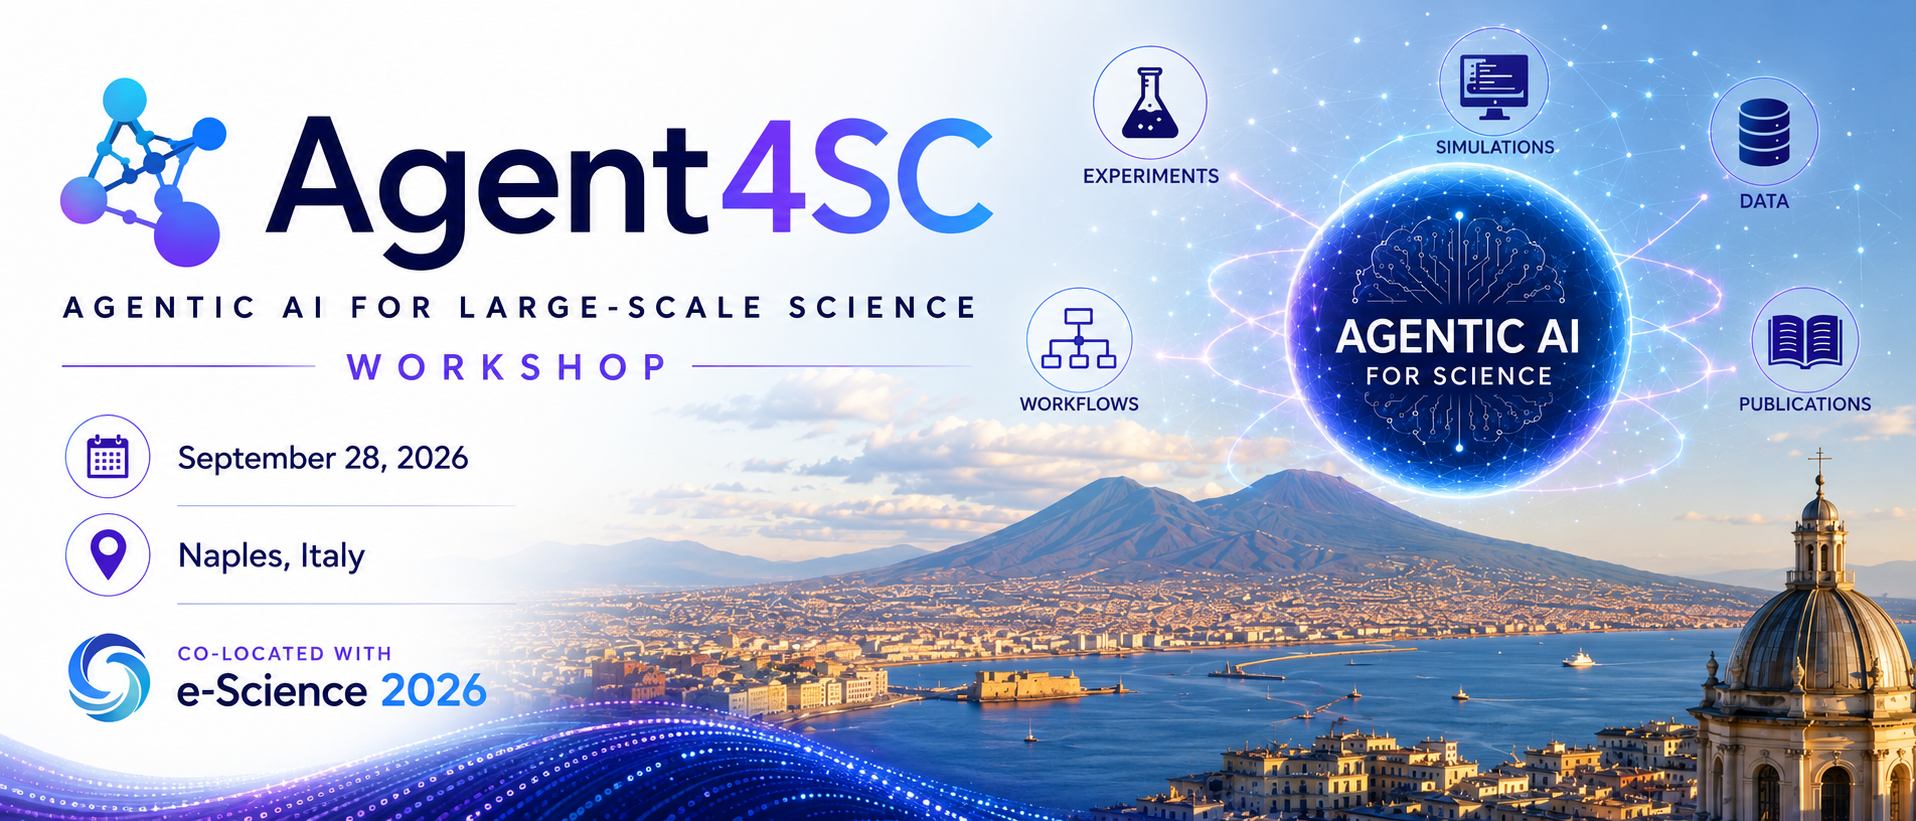
\includegraphics[width=\linewidth]{banner_amal.png}

\vspace{0.45cm}

% ============================================================
%  IMPORTANT DATES  (colored box)
% ============================================================
\begin{mdframed}[
  backgroundcolor=lightlavender,
  linecolor=accent,
  linewidth=1.5pt,
  leftmargin=0pt, rightmargin=0pt,
  innerleftmargin=14pt, innerrightmargin=14pt,
  innertopmargin=10pt, innerbottommargin=10pt,
  roundcorner=4pt
]
\begin{center}
  {\large\textbf{\textcolor{navyblue}{Important Dates}}}
\end{center}
\vspace{2pt}
\begin{center}
\renewcommand{\arraystretch}{1.4}
\begin{tabular}{l@{\hspace{2cm}}l}
  \textcolor{midgray}{Papers Due}               & \textbf{\textcolor{accent}{July 21, 2026}} \\
  \textcolor{midgray}{Notification of Acceptance} & \textbf{August 3, 2026}  \\
  \textcolor{midgray}{Camera-Ready Papers}        & \textbf{August 10, 2026} \\
  \textcolor{midgray}{Workshop}                   & \textbf{IEEE eScience 2026} \\
\end{tabular}
\end{center}
\vspace{4pt}
\begin{center}
  {\small Submit via \textbf{EasyChair}:
    \url{https://easychair.org/my/conference?conf=escience2026}}\\[2pt]
  {\small Select track: \textit{\textbf{1st Workshop on Agentic AI for Large-scale Science}}}
\end{center}
\end{mdframed}

\vspace{0.4cm}

% ============================================================
%  ABOUT
% ============================================================
{\color{navyblue}\large\textbf{About AGENT4SC}}
\ThinRule\vspace{4pt}

Agentic AI is rapidly moving from ``chat with tools'' prototypes to autonomous
systems that can reason, plan, coordinate, and act across complex digital
research ecosystems. For the eScience community, this represents the emergence
of a new \textbf{control plane} for computational and data-driven research.

Agents can request allocations, launch ensembles, steer workflows, move
PB-scale datasets, trigger experiment/compute co-scheduling, and generate
decisions that impact scientific validity---spanning the computing continuum
from instruments and autonomous laboratories to simulations, data centers,
cloud systems, and leadership-class HPC.

\textbf{AGENT4SC} provides a dedicated forum to advance \textbf{scalable
architectures, cross-continuum coordination, evaluation frameworks, safety and
verification strategies, provenance, and observability mechanisms} before
agentic systems become embedded in production research workflows.

\vspace{10pt}

% ============================================================
%  TOPICS
% ============================================================
{\color{navyblue}\large\textbf{Topics of Interest}}
\ThinRule\vspace{4pt}

We welcome contributions on, but not limited to:

\begin{itemize}[leftmargin=16pt, itemsep=1pt, topsep=2pt]
  \item System architectures \& design principles for agentic AI at scale
  \item Agentic AI for the edge--cloud--HPC continuum
  \item Agent memory \& long-horizon reasoning under compute constraints
  \item Data \& metadata architectures (vector stores, knowledge graphs)
  \item Human-in-the-loop \& oversight for long autonomous campaigns
  \item Provenance, observability, auditability, and reproducibility
  \item Safety, security \& accountability in production science
  \item Hallucination detection, mitigation, and recovery
  \item Performance modeling under realistic scientific workloads
  \item Interoperability \& standardization (interfaces, protocols, schemas)
  \item Cross-platform scheduling under agent-driven control
  \item Real-world experience reports from large-scale deployments
\end{itemize}

\vspace{10pt}

% ============================================================
%  PAPER FORMATS
% ============================================================
{\color{navyblue}\large\textbf{Paper Formats}}
\ThinRule\vspace{4pt}

\begin{itemize}[leftmargin=16pt, itemsep=3pt, topsep=2pt]
  \item \textcolor{accent}{\textbf{4 pages}} --- \textbf{Short Paper}: work-in-progress (\emph{not including references})
  \item \textcolor{accent}{\textbf{8 pages}} --- \textbf{Full Paper}: complete research (\emph{not including references})
\end{itemize}

\vspace{10pt}

% ============================================================
%  SUBMISSION GUIDELINES
% ============================================================
{\color{navyblue}\large\textbf{Submission Guidelines}}
\ThinRule\vspace{4pt}

\begin{itemize}[leftmargin=16pt, itemsep=1pt, topsep=2pt]
  \item Papers must be written in \textbf{English} and formatted per
        \href{https://www.escience-conference.org/2026/call-for-papers}{IEEE eScience 2026 author guidelines}
  \item All papers receive \textbf{at least three} peer reviews from the Program Committee
  \item Accepted papers published in the official \textbf{eScience 2026 workshop proceedings}
  \item Authors are encouraged to include reproducibility information about
        software, data artifacts, and AI assistants used
\end{itemize}

\vspace{10pt}

% ============================================================
%  ORGANIZERS & STEERING
% ============================================================
{\color{navyblue}\large\textbf{Organizers}}
\ThinRule\vspace{6pt}

\begin{tabular}{ll}
  \textbf{Amal Gueroudji} &
    \textcolor{midgray}{Argonne National Laboratory, USA} \quad
    \href{mailto:agueroudji@anl.gov}{agueroudji@anl.gov} \\[4pt]
  \textbf{Renan Souza} &
    \textcolor{midgray}{Oak Ridge National Laboratory, USA} \quad
    \href{mailto:souzar@ornl.gov}{souzar@ornl.gov} \\
\end{tabular}

\vspace{10pt}

{\color{navyblue}\large\textbf{Steering Committee}}
\ThinRule\vspace{4pt}

{\small
\begin{tabular}{ll}
  Rosa Filgueira      & University of St Andrews, UK \\[2pt]
  Rafael Ferreira da Silva & Oak Ridge National Laboratory, USA \\[2pt]
  Kyle Chard          & Argonne National Laboratory, USA \\[2pt]
  Patrick Widener     & Oak Ridge National Laboratory, USA \\
\end{tabular}
}

% ============================================================
%  FOOTER
% ============================================================
\vfill
\noindent{\color{ruleblue}\rule{\linewidth}{0.5pt}}
\vspace{4pt}
\begin{center}
  {\small\textcolor{midgray}{%
    \textbf{Website:} \url{https://agent4sc.github.io}
    \quad|\quad
    \textbf{Submission:} \url{https://easychair.org/my/conference?conf=escience2026}
    \quad|\quad
    \textbf{Contact:} \href{mailto:agueroudji@anl.gov}{agueroudji@anl.gov}
  }}
\end{center}

\end{document}
